
\documentclass{article}%
\usepackage{hyperref}
\usepackage{geometry}
\usepackage{sectsty}%
\usepackage{amsfonts}
\usepackage{amssymb}
\usepackage{graphicx}
\usepackage[export]{adjustbox}
\usepackage{wrapfig}
\usepackage{textpos}
\usepackage{enumitem}
\usepackage{verbatim}



\usepackage[T1]{fontenc}
\usepackage{lmodern}



\providecommand{\U}[1]{\protect\rule{.1in}{.1in}}
\def\name{Lucas Rentschler}
\hypersetup{
colorlinks = true,
urlcolor = black,
pdfauthor = {\name},
pdfkeywords = {experimental economics, game theory, applied microeconomics},
pdftitle = {\name: Curriculum Vitae},
pdfsubject = {Curriculum Vitae},
pdfpagemode = UseNone
}
\geometry{
body={7in, 9.5in},
left=.7in,
top=.7in
}
\pagestyle{myheadings}
\markright{\name}
\thispagestyle{empty}
\sectionfont{\rmfamily\mdseries\LARGE}
\subsectionfont{\rmfamily\mdseries\scshape\large}
\subsubsectionfont{\rmfamily\mdseries\scshape\small}
\setlength\parindent{0em}
\renewenvironment{itemize}{
\begin{list}{}{
\setlength{\leftmargin}{1.5em}
}
}{
\end{list}
}
\setcounter{secnumdepth}{0}
\begin{document}

%Place name at left
%{\huge Lucas Rentschler}
%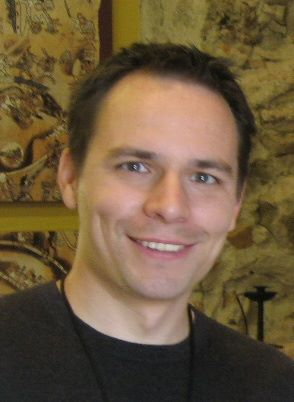
\includegraphics[width=3cm,right]{cvphoto.jpg}
%Alternatively, print name centered and bold:
%\centerline{\huge \bf \name}


%\begin{minipage}[t]{0.5\textwidth}
%\href{http://www.ufm.edu/}{Universidad Francisco Marroqu\'{i}n} \\
%\href{http://www.fce.ufm.edu/}{Facultad de Ciencias Econ\'{o}micas} \\
%Citizenship: United States
%\end{minipage}

{\Huge Lucas Rentschler}\\


\begin{textblock}{0.9}[0.5,0.5](11,.6)
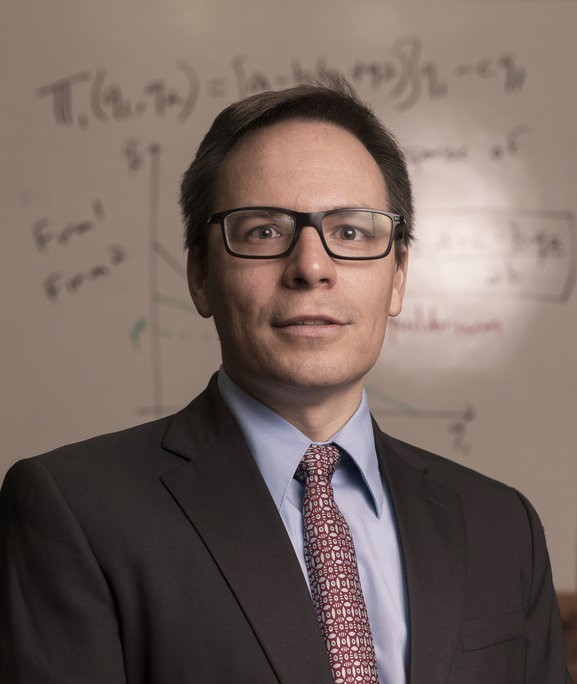
\includegraphics[width=3cm]{cvphototie.jpg}
\end{textblock}

Phone: 435 797 2397 \\
Email: \href{mailto:lucas.rentschler@usu.edu}{\tt lucas.rentschler@usu.edu} \\
%Skype: lucas.rentschler\\
Webpage: \href{lucasrentschler.com}{www.lucasrentschler.com}\\
%Citizenship: United States


\section*{Education}

\begin{itemize}
\item Ph.D. Economics, Texas A\&M University, 2010.

\item B.S. English and Economics, Weber State University, 2004.

\end{itemize}

\section*{Fields of Specialization}

Industrial Organization, Economic Theory, Development Economics, Law and Economics

\section*{Academic Positions}

\begin{itemize}
\item Assistant Professor at Utah State University, August 2017 - Present.
\item Research Affiliate at the Economic Science Institute at Chapman University, June 2017 - Present.
\item Research Professor at Chapman University, January 2017 - May 2017.
\item Professor of Economics at Universidad Francisco Marroqu\'{\i}n, June 2010 - February 2017.
\item Senior Research Fellow at Centro Vernon Smith de Econom\'{i}a Experimental, June 2013 - February 2017. 
\item Research Fellow at Centro Vernon Smith de Econom\'{i}a Experimental, June 2010 - June 2013. 
\end{itemize}

\section*{Research}

\subsection*{Journal Articles}


\begin{itemize}

\item ``Stag Hunt Contests and Alliance Formation,'' with James Boudreau and Shane Sanders. \textit{Public Choice,} 2018.

\item ``Valuation Structure in Incomplete Information Contests: Experimental Evidence,'' with Diego Aycinena and Rimvydas Baltaduonis. \textit{Public Choice,} 2018.

\item ``Discounting and Digit Ratio: Low 2D:4D Predicts Patience
for a Sample of Females,'' with Diego Aycinena. \emph{Frontiers in Behavioral Neuroscience,} 2017.

\item ``An Experiment on Asymmetric Information in First-Price Common-Value Auctions: The Blessed Winner,'' with
\href{http://www.bgrosskopf.com}{Brit Grosskopf} and \href{http://econweb.tamu.edu/rsarin}{Rajiv Sarin}. \emph{Games and Economic Behavior,} 2017.

\item ``Revenue in Auctions with Endogenous Participation and an Uncertain Number of Bidders: Experimental Evidence,'' with
\href{www.diegoaycinena.com}{Diego Aycinena}. \emph{Experimental Economics,} 2017.

\item ``Informed Entry in Auctions,'' with
\href{www.diegoaycinena.com}{Diego Aycinena} and Hern\'{a}n Bejarano. \emph{International Journal of Game Theory,} 2017.

\item ``Two-bidder All-Pay Auctions with Interdependent Valuations, Including the Highly Competitive Case,'' with \href{http://www.uea.ac.uk/economics/people/profile/t-turocy}{Theodore Turocy}, \emph{Journal of Economic Theory,} 2016.

\item ``Fraying of the Ties that Bind: Community-Level Financial Institutions and HIV/AIDS with Evidence from KwaZulu Natal, South Africa,'' with Benjamin Linkow, \emph{Journal of African Economies,} 2016.

\item ``Common-Value Procurement Auctions with Renegotiation,'' with \href{http://public.gettysburg.edu/~rbaltadu/}{Rimvydas Baltaduonis}, \emph{Theoretical Economics Letters,} 2014.

\item ``Valuation Structure in First-Price and Least-Revenue Auctions: An Experimental Investigation,'' with
\href{www.diegoaycinena.com}{Diego Aycinena} and \href{http://public.gettysburg.edu/~rbaltadu/}{Rimvydas Baltaduonis}, \emph{Experimental Economics,} 2014.

\item ``Risk Preferences and Prenatal Exposure to Sex Hormones for Ladinos,'' with
\href{www.diegoaycinena.com}{Diego Aycinena} and
\href{http://public.gettysburg.edu/~rbaltadu/}{Rimvydas Baltaduonis,} \emph{PLoS One,} 2014.

\end{itemize}
\subsection*{Submitted}
\begin{itemize}


\item ``Demand for Intra-Household Control, Risk and Discounting for Recipients of Conditional Cash Transfers,'' with \href{www.diegoaycinena.com}{Diego Aycinena}, Szabolcs Blazsek and Betzy Sandoval. \textit{Revision requested, Journal of Applied Economics.}

\item ``Priming the Jury by Asking for Donations: An Empirical and Experimental Study,'' with Jason Aimone and Charles North. \textit{Revision requested, Journal of Economic Behavior and Organization.}

\item ``Endogenous Entry in Contests with Incomplete Information: Theory and Experiments,'' with Diego Aycinena. \textit{Revision requested, European Journal of Political Economy.}

\item ``Intertemporal Choice Experiments and Large-Stakes Behavior,'' with Diego Aycinena, Szabolcs Blazsek and Charles Sprenger.

\end{itemize}



\subsection*{Working Papers}
\begin{itemize}
\item ``Tu Mihi Soli Places: An Experiment on the Competitiveness of All-Pay Auctions with Private Information,'' with Theodore Turocy.

\item ``All-Pay Auctions with Noise.'' with with James Boudreau and Shane Sanders. 

\item ``Asymmetric Information in Contests: Theory and
Experiments,'' with \href{http://www.bgrosskopf.com}{Brit
Grosskopf} and \href{http://econweb.tamu.edu/rsarin}{Rajiv Sarin}.

\item ``Incumbency in Imperfectly Discriminating
Contests.'' \\ \hspace*{1cm}

\end{itemize}

\subsection*{Other}
\begin{itemize}

\item ``What Can Experimental Economists Learn from Adam Smith?,'' with Diego Aycinena, \emph{UFM Companion to Adam Smith,} 2016.

\item ``Book Review of \underline{The Pursuit of Justice: Law and Economics of Legal Institutions},'' \emph{Laissez-Faire,} 2012.

\item ``Lex Oppia : An Ancient Example of the Persistence of Emergency Powers,'' with
Christopher Dawe, \emph{Laissez-Faire,} 2011.

\end{itemize}


\subsection*{Works in Progress}
\begin{itemize}



\item ``Asymmetric Information and Equilibrium Selection,'' with \href{www.diegoaycinena.com}{Diego Aycinena}
and \href{http://public.gettysburg.edu/~rbaltadu/}{Rimvydas Baltaduonis}. 
\begin{itemize}\vspace{-.24cm}
\item \textit{Data collection complete, data analysis in progress.}
\end{itemize}

\item ``Injunctive and Descriptive Social Norms regarding Cheating: Cross Cultural Evidence,'' with Diego Aycinena, Benjamin Beranek and Jonathan Schulz. 
\begin{itemize}\vspace{-.24cm}
\item \textit{Data collection complete, data analysis in progress.}
\end{itemize}

\item ``Juror Decision Making and the Timing of Information Acquisition,'' with Andrei Gomberg, Diego Aycinena and Alex Elbittar. \begin{itemize}\vspace{-.24cm}
\item \textit{Data collection complete, data analysis in progress.}
\end{itemize}

\item ``Leveling the Playing Field,'' with Daniel Kovenock. 
\begin{itemize}\vspace{-.24cm}
\item \textit{Data collection complete, data analysis in progress.}
\end{itemize}


\item ``Social Norms and Third Party Punishment: The Role of Status,'' with Diego Aycinena. 
\begin{itemize}\vspace{-.24cm}
\item \textit{Data collection in progress.}
\end{itemize}


\item ``Enforcement,'' with Jason Aimone, Vernon Smith and Bart Wilson. 
\begin{itemize}\vspace{-.24cm}
\item \textit{Design in progress.}
\end{itemize}

\end{itemize}

\section*{Teaching Experience}

\subsection*{Utah State University}
\begin{itemize}
\item Mathematical Economics, Fall 2017, Spring 2018, Fall 2018.
\item Econometrics, Spring 2018, Fall 2018. 
\end{itemize}


\subsection*{Universidad Francisco Marroqu\'{\i}n}

\begin{itemize}

\item Econometrics, Spring 2014, Spring 2015.

\item Intermediate Microeconomics, Spring 2012, Spring 2013, Spring 2014.

\item Advanced Macroeconomics, Fall 2012, Fall 2014.

\item Principles of Microeconomics, Spring 2011, Spring 2012, Spring 2013, Spring 2016.

\item Industrial Organization, Spring 2011, Spring 2015, Spring 2016.

\item Principles of Macroeconomics, Fall 2010, Fall 2011, Fall 2015, Fall 2016.

\item Game Theory, Fall 2010, Fall 2012, Fall 2013, Fall 2014, Fall 2015, Fall 2016.
\end{itemize}

\subsection*{Texas A\&M University}

\begin{itemize}
\item Game Theory, Fall 2009.

\item Principles of Microeconomics, Fall 2006, Spring 2007, Summer 2007, Spring 2008.

\item Intermediate Microeconomics, Fall 2007.
\end{itemize}

\section*{Professional Activities}

\subsection*{Service}

\begin{itemize}
\item Co-Organizer, North American Economic Science Association Meetings, 2018. 

\item Co-Organizer, Antigua Experimental Economics Workshop, 2018. 

\item Co-Organizer, Antigua Experimental Economics Conference, 2018.

\item Co-Organizer, Center for Growth and Opportunity Experimental Economics Workshop, 2017. 

\item Co-Organizer, Antigua Experimental Economics Conference, 2017. 

\item Co-Organizer, Antigua Experimental Economics Conference, 2016. 

\item Co-Organizer, Antigua Experimental Economics Conference, 2015. 

\item Co-Organizer, Antigua Experimental Economics Workshop, 2015. 

\item Co-Organizer, Antigua Experimental Economics Conference, 2014. 

\item Co-Organizer, Antigua Experimental Economics Workshop, 2014. 

\item Co-Organizer, Guatemala Experimental Economics High School Workshop, 2013.

\item Co-Organizer, Antigua Experimental Economics Conference, 2012. 

\item Co-Organizer, Antigua Experimental Economics Workshop, 2012. 

\item Co-Organizer, Guatemala Experimental Economics High School Workshop, 2012.

\item Faculty Advisor, Economics Honor Society, Universidad Francisco Marroqu\'{\i}n, July 2012 - December 2016.

\end{itemize}

\subsection*{Awards and Grants}

\begin{itemize}
\item International Foundation for Research in Experimental Economics support for the Bogot\'{a} Experimental Economics Workshop and Conference, with Diego Aycinena, $\$14800$, 2017.
\item International Foundation for Research in Experimental Economics support for the $5^{th}$ Antigua Experimental Economics Workshop and Conference, with Diego Aycinena, $\$14800$, 2016.
\item UFM Faculty Research Grant, $\$1000$, 2016.
\item Charles Koch Foundation Grant for Criminal Justice and Policing Reform, with Jason Aimone and Charles  North, $\$4500$, 2015.
\item UFM Faculty Research Grant, $\$1500$, 2015.
\item International Foundation for Research in Experimental Economics support for the $4^{th}$ Antigua Experimental Economics Workshop and Conference, with Diego Aycinena, $\$14800$, 2015.
\item International Foundation for Research in Experimental Economics support for the $3^{rd}$ Antigua Experimental Economics Workshop and Conference, with Diego Aycinena, $\$14800$, 2014.
\item International Foundation for Research in Experimental Economics support for the $2^{nd}$ Antigua Experimental Economics Workshop and Conference, with Diego Aycinena, $\$14800$, 2013.
\item International Foundation for Research in Experimental Economics support for the $1^{st}$ Antigua Experimental Economics Workshop and Conference, with Diego Aycinena, $\$14800$, 2012.
\item International Foundation for Research in Experimental Economics support for Experiments on Auctions with Entry, with Diego Aycinena, $\$10000$, 2011.

\item UFM Faculty Research Grant, with Diego Aycinena, $\$5000$, 2011.

\item Graduate Assistantship, Texas A\&M University, Fall 2004 - Fall 2009.

\item Outstanding Teaching Award, Texas A\&M University, 2008.

\end{itemize}

\subsection*{Professional Memberships}

\begin{itemize}
\item American Economic Association.

\item Economic Science Association.

\item Guatemalan Econometrics Study Group.


\end{itemize}

\subsection*{Invited Presentations}


\begin{itemize}
%\setlength\itemsep{1em}

\item Texas A\&M University, 2016.
\begin{itemize}\vspace{-.24cm}
\item \textit{Paper presented:} ``Tu Mihi Soli Places: An Experiment on the Competitiveness of All-Pay Auctions with Private Information.''
\end{itemize}

\item Universidad del Rosario, 2016.
\begin{itemize}\vspace{-.24cm}
\item \textit{Paper presented:} ``Tu Mihi Soli Places: An Experiment on the Competitiveness of All-Pay Auctions with Private Information.''
\end{itemize}

\item University of Exeter, 2015.
\begin{itemize}\vspace{-.24cm}
\item \textit{Paper presented:} ``Feedback Response In Competitive Environments.''
\end{itemize}

\item Weber State University, 2015.
\begin{itemize}\vspace{-.24cm}
\item \textit{Paper presented:} ``Demand for Intra-Household Control, Risk and Discounting for Recipients of Conditional Cash Transfers.''
\end{itemize}

\item University of Michigan, 2012.
\begin{itemize}\vspace{-.24cm}
\item \textit{Paper presented:}  ``What Drives Over-Expenditure of Effort in Contests? An Experimental Investigation.''
\end{itemize}

\item Universidad Francisco Marroqu\'{i}n, 2010.
\begin{itemize}\vspace{-.24cm}
\item \textit{Paper presented:} ``An Experimental Investigation of Asymmetric Information in Common-Value Auctions.''
\end{itemize}

\end{itemize}

%\begin{comment}

\subsection*{Conference Presentations}

\begin{itemize}

\item International Economic Science Association Conference, Berlin, 2018.
\begin{itemize}\vspace{-.24cm}
\item \textit{Paper presented:} ``Tilting the Playing Field in All-Pay Auctions.''
\end{itemize}

\item Association of Private Enterprise Education Conference, Las Vegas, 2018.
\begin{itemize}\vspace{-.24cm}
\item \textit{Paper presented:} ``Auctions with Endogenous Participation and an Uncertain Number of Bidders: Experimental Evidence.''
\end{itemize}

\item Public Choice Society Meetings, Charleston, 2018.
\begin{itemize}\vspace{-.24cm}
\item \textit{Paper presented:} ``All-Pay Auctions with Noise.''
\end{itemize}

\item 28th International Conference on Game Theory at the Stony Brook Center for Game Theory, Stony Brook, 2017.
\begin{itemize}\vspace{-.24cm}
\item \textit{Paper presented:} ``Valuation Structure in Incomplete Information Contests: Experimental Evidence.''
\end{itemize}


\item International Economic Science Association Conference, San Diego, 2017.
\begin{itemize}\vspace{-.24cm}
\item \textit{Paper presented:} ``Tu Mihi Soli Places: An experiment on the Competitiveness of All-Pay Auctions with Private Information.''
\end{itemize}


\item CESifo Venice Summer Institute 2017: Dynamics of Conflict - Results from Theory and Experiments, Venice, 2017.
\begin{itemize}\vspace{-.24cm}
\item \textit{Paper presented:} ``Entry in all-pay auctions with incomplete information: Theory and Experiments.''
\end{itemize}

\item Society for the Advancement of Economic Theory Meetings, Rio de Janeiro, 2016.
\begin{itemize}\vspace{-.24cm}
\item \textit{Paper presented:} ``Tu Mihi Soli Places: An experiment on the Competitiveness of All-Pay Auctions with Private Information.''
\end{itemize}


\item University of East Anglia CBESS Conference on Contest Theory, Norwich, 2016.
\begin{itemize}\vspace{-.24cm}
\item \textit{Paper presented:} ``Endogenous entry in contests with incomplete information: Theory and experiments.''
\end{itemize}


\item Association of Private Enterprise Education Conference, Las Vegas, 2016.
\begin{itemize}\vspace{-.24cm}
\item \textit{Paper presented:} ``Corporate Social Responsibility: Consumer Oversight and the Substitutability of Giving Channels.''
\end{itemize}


\item Public Choice Society Meetings, Fort Lauderdale, 2016.
\begin{itemize}\vspace{-.24cm}
\item \textit{Paper presented:} ``Two-Bidder All-Pay Auctions with Interdependent Valuations, Including the Highly Competitive Case.''
\end{itemize}


\item North American Economic Science Association Conference, Dallas, 2015.
\begin{itemize}\vspace{-.24cm}
\item \textit{Paper presented:} ``Corporate Social Responsibility: Consumer Oversight and the Substitutability of Giving Channels.''
\end{itemize}

\item Antigua Experimental Economics Conference, Antigua, 2015.
\begin{itemize}\vspace{-.24cm}
\item \textit{Paper presented:} ``Feedback Response In Competitive Environments.''
\end{itemize}

\item North American Economic Science Association Conference, Ft. Lauderdale, 2014.
\begin{itemize}\vspace{-.24cm}
\item \textit{Paper presented:} ``Two-Bidder All-Pay Auctions with Private Signals: Experimental Evidence.''
\end{itemize}

\item Association of Private Enterprise Education Conference, Las Vegas, 2014.
\begin{itemize}\vspace{-.24cm}
\item \textit{Paper presented:} ``All-Pay Auctions with Endogenous Entry.''
\end{itemize}

\item Antigua Experimental Economics Conference, Antigua, 2014.
\begin{itemize}\vspace{-.24cm}
\item \textit{Paper presented:} ``All-Pay Auctions with Endogenous Entry.''
\end{itemize}

\item International Economic Science Association Conference, Zurich, 2013.
\begin{itemize}\vspace{-.24cm}
\item \textit{Paper presented:} ``Endogenous Entry in Contests With Incomplete Information: Theory and Experiments.''
\end{itemize}

\item Association of Private Enterprise Education Conference, Hawaii, 2013.
\begin{itemize}\vspace{-.24cm}
\item \textit{Paper presented:} ``What Drives Over-Expenditure of Effort in Contests? An Experimental Investigation.''
\end{itemize}

\item Antigua Experimental Economics Conference, Antigua, 2012.
\begin{itemize}\vspace{-.24cm}
\item \textit{Paper presented:} ``What Drives Over-Expenditure of Effort in Contests? An Experimental Investigation.''
\end{itemize}

\item International Economic Science Association Conference, New York, 2012.
\begin{itemize}\vspace{-.24cm}
\item \textit{Paper presented:} What Drives ``Over-Expenditure of Effort in Contests? An Experimental Investigation.''
\end{itemize}

\item North American Economic Science Association Conference, Tucson, 2011.
\begin{itemize}\vspace{-.24cm}
\item \textit{Paper presented:} ``Perfectly Discriminating Contests with Incomplete Information.''
\end{itemize}

\item International Economic Science Association Conference, Chicago, 2011.
\begin{itemize}\vspace{-.24cm}
\item \textit{Paper presented:} ``Asymmetric Information in Contests: Theory and Experiments.''
\end{itemize}

\item Association of Private Enterprise Education Conference, Nassau, 2011.
\begin{itemize}\vspace{-.24cm}
\item \textit{Paper presented:} ``Asymmetric Information in
Common-Value First-Price Auctions: Experimental Evidence.''
\end{itemize}

\item North American Economic Science Association Conference, Tucson, 2010.
\begin{itemize}\vspace{-.24cm}
\item \textit{Paper presented:} ``Asymmetric Information in
Common-Value First-Price Auctions: Experimental Evidence.''
\end{itemize}

\item International Economic Science Association Conference, Washington D.C., 2009.
\begin{itemize}\vspace{-.24cm}
\item \textit{Paper presented:} ``An Experimental Investigation of Asymmetric Information in Common-Value
Auctions.''
\end{itemize}

\item North American Economic Science Association Conference, Tucson, 2008.
\begin{itemize}\vspace{-.24cm}
\item \textit{Paper presented:} ``An Experimental
Investigation of Asymmetric Information in Common-Value Auctions.''
\end{itemize}
\end{itemize}

%\end{comment}

\subsection*{Refereeing}

\begin{itemize}
\item B.E. Journal of Economic Analysis and Policy
\item Economic Inquiry
\item Economic Theory
\item Games and Economic Behavior
\item International Journal of Game Theory
\item Journal of Economic Behavior \& Organization
\item Journal of Economic Psychology
\item Management Science
\item Optimization Methods and Software
\item Public Choice
\end{itemize}
\newpage
\clearpage

\begin{comment}
\thispagestyle{empty}

\section*{References for Lucas Rentschler}

\begin{minipage}[t]{0.8\textwidth}
\begin{itemize}
\item Rajiv Sarin \\ Professor of Economics \\ University of Exeter \\
  +44 (0) 139 272 5975 \\
  \href{mailto:r.sarin@exeter.ac.uk}{\tt r.sarin@exeter.ac.uk}
\item Brit Grosskopf \\ Professor of Economics \\ University of Exeter \\
  +44 (0) 139 272 5976 \\
  \href{mailto:b.grosskopf@exeter.ac.uk}{\tt b.grosskopf@exeter.ac.uk }
\item Szabolcs Blazsek \\ Professor of Economics\\School of Business \\Universidad Francisco Marroqu\'{\i}n \\
  +502 2338 7788   \\
  \href{mailto:sblazsek@ufm.edu}{\tt sblazsek@ufm.edu}
\item Rimvydas Baltaduonis \\ Associate Professor of Economics \\ Gettysburg College \\
  +1 717 337 6671 \\
  \href{mailto:rbaltadu@gettysburg.edu}{\tt rbaltadu@gettysburg.edu}
\end{itemize}
\end{minipage}

\end{comment}


\end{document}
